\chapter{Introduction}
\label{cha:intro}


% SECTION 1
\section{Microbial ecology}

   \subsection{Microbial communities: structure (\textit{who}) \& function (\textit{what})}

      Microbial ecology studies the interactions of the various microbial taxa with their environment, 
      as well as those among them or/and between them and their host~\cite{isme}.
      Microbes, i.e. Bacteria, Archaea and small Eukaryotes, 
      and the communities they form are part of almost any known ecosystem type 
      and they impact global ecosystem functions to a great extent~\citep{falkowski2008microbial}.
      Microbes are considered to be omnipresent~\citep{falkowski2008microbial}; 
      it was only recently (~\citeyear{belilla2019hyperdiverse}) that scientists discovered for the first time 
      a place on Earth where no microbial forms of life are present~\cite{belilla2019hyperdiverse}.
      Extremely low pH, high salt and high temperature had to be 
      at the same place at the same time to stop microbes~\citep{belilla2019hyperdiverse}.
      Despite the extensive studies of the scientific community, 
      less than 1\% of the microbial species on Earth are currently identified~\ref{isme}.

      (apo afoulophdh)

      Based on the type of energy source (Figure 1.1A), on the carbon source (Figure 1.1B)
      and the electron source (Figure 1.1C), microorganisms can be divided in certain
      categories. Practically, all these terms can be combined; for example,
      chemolithoautotrophic bacteria, e.g. nitrifying and sulfur-oxidizing bacteria, as well
      as photoautotrophic bacteria, e.g. purple bacteria and Green sulfur bacteria, can be
      found in nature. Also, mixotrophy can be either photochemotrophic (e.g. SAR11,
      SAR86) or lithoorganotrophic (e.g. many marine Alphaproteobacteria).


      The metabolic pathways that are catalyzed by microbes include all the major
      elements that are the necessary prerequisites for the construction of biological
      macromolecules, i.e. carbon, hydrogen, oxygen, phosphorus, nitrogen and sulfur
      (Falkowski et al., 2008). Despite the fact that, over the last decades, our knowledge
      on the specific enzymatic reactions that regulate these pathways has increased,
      there are still more to be discovered (Arrigo, 2005) especially in the light of projected
      climate changes (Singh et al., 2010).





      Their abundance \citep{bar2018biomass}, versatility \citep{rees2017improving} 
      and interactions \citep{rottjers2018hairballs}. 



      Microbial ecologists also investigate the role of microbial taxa in 
      biogeochemical cycles~\cite{falkowski2008microbial} and their interaction 
      with anthropogenic effects e.g. pollution and climate change~\cite{cavicchioli2019scientists}.

      In Figure~\ref{fig:co2} the contirbution of microbial communities 
      in the cycle of CO\_2 is shown. 



       
      \begin{figure}[h]
         \centering
         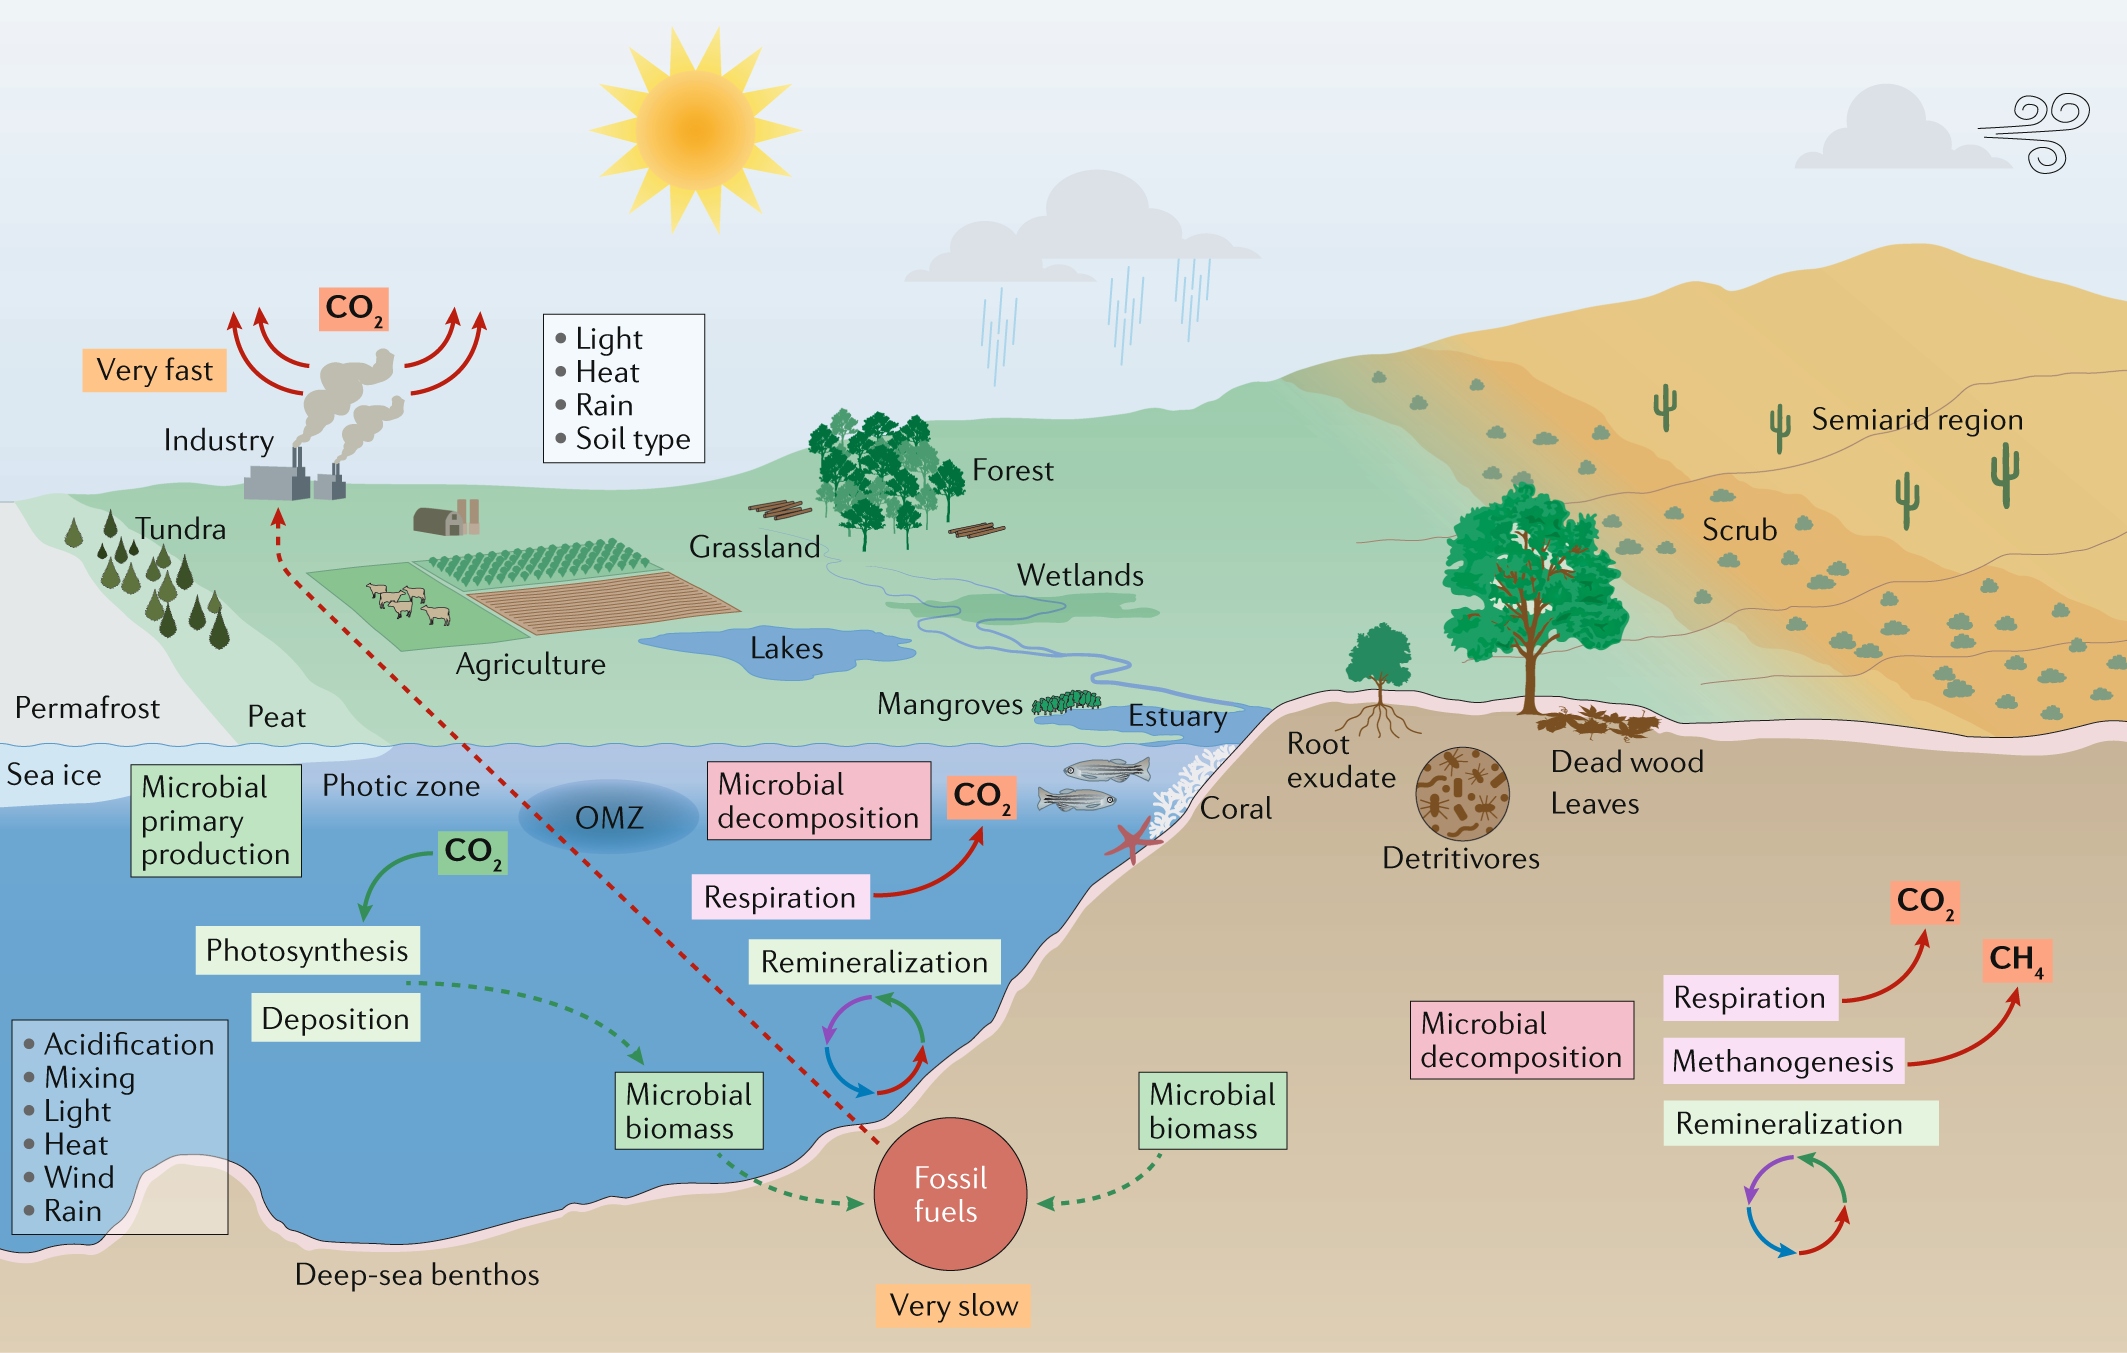
\includegraphics[width=135mm]{figures/ecosystem_functioning.png}
         \caption[The cycle of C and the role of microbial communiites]{Marine microbial communities contribute to CO$_2$ sequestration, nutrients recycle and thus to the release of CO$_2$ to the atmosphere. 
         Soil microbial communities decomposers organic matter and release nutrients in the soil 
         from \citep{cavicchioli2019scientists} doi: \href{https://doi.org/10.1038/s41579-019-0222-5}{10.1038/s41579-019-0222-5}, under \href{http://creativecommons.org/licenses/by/4.0 license}{Creative Commons Attribution 4.0 International License}
         }
         \label{fig:co2}
      \end{figure}







      % This is copy paste from Wikipedia about hydrothermal vent microb comm
      % https://www.wikiwand.com/en/Hydrothermal_vent_microbial_communities
      Microbial communities at hydrothermal vents mediate the transformation of energy 
      and minerals produced by geological activity into organic material. 
      Organic matter produced by autotrophic bacteria is then used to support the upper trophic levels. 
      The hydrothermal vent fluid and the surrounding ocean water is rich in elements such as iron, 
      manganese and various species of sulfur including sulfide, sulfite, sulfate, elemental sulfur from 
      which they can derive energy or nutrients.[8] Microbes derive energy by oxidizing or reducing elements. 
      Different microbial species use different chemical species of an element in their metabolic processes. 
      For example, some microbe species oxidize sulfide to sulfate and another species will reduce sulfate to elemental sulfur. 
      As a result, a web of chemical pathways mediated by different microbial species transform elements such as 
      carbon, sulfur, nitrogen, and hydrogen, from one species to another. 
      Their activity alters the original chemical composition produced by geological activity of the hydrothermal vent environment.[9]


      metabolic interactions --> auxotrophy, prototrophy Giri et al (2021)




   \subsection{Microbial interactions: unravelling the microbiome}

      Microbial interactions play a fundamental role in deciphering the underlying mechanisms that govern ecosystem functioning. 
      Co-occurrence networks have been widely used for inferring microbial associations or/and interactions from metagenomic data. 
      However, spurious associations and tool-dependence confine the network inference. 


      \textbf{types of interactions} \\
      
      (from Karoline's~\cite{faust2012microbial})
      mutualism: a win–win relationship that is known as mutualism
      cross-feeding (also known as syntrophy), in which two species exchange metabolic products to the benefit of both

      In commensalistic relationships, one partner benefits without helping or harming the other. Commensalism is often found in biodegradation, in which commensals cross-feed on compounds that are produced by other community members (for example, in cellulose degradation)

      competition between microorganism (a loss–loss relationship)
      On the basis of
      these observations, Gause formulated his law of competitive exclusion, which states that two species with
      similar niches exclude each other

      Amensalism — in which one partner is harmed without any advantage to the other — occurs, for example,
      when metabolic by-products of a microbial species
      alter the environment to the detriment of other microorganisms (for example, lactobacilli lowering the pH
      of the surrounding environment). I



      \subsubsection*{Reverse ecology}


         - genotype - phenotype relationship \\

         (from Roie Levy and Elhanan Borenstein~\cite{levy2012reverse})
         Reverse Ecology—an emerging new frontier in Evolutionary Systems Biology—aims
         to extract this information and to obtain novel insights into an organism’s ecology.
         The Reverse Ecology framework facilitates the translation of high-throughput
         genomic data into large-scale ecological data, and has the potential to transform
         ecology into a high-throughput field




         (from RevEcoR publication~\cite{cao2016revecor})
         A systematic approach for describing microbiome ecologies and the interactions between microbiota is lacking. 
         To address this challenge, a systems biology approach called \textit{reverse ecology} has been developed 
         to study the complex interactions and species composition of microbial communities [4]. 
         Reverse ecology uses genomics to study community ecology with no a priori assumptions about the organisms under consideration. 
         Researchers can use it to infer the ecology of a system directly from genomic information. 
         The reverse ecology framework uses advances in systems biology and genomic metabolic modeling and 
         the system-level analysis of complex biological networks to predict the ecological traits of poorly studied microorganisms, 
         their interactions with other microorganisms, and the ecology of microbial communities. 
         Several studies have applied this approach to investigate the interactions between microorganisms 
         and their surroundings on a large scale [4, 5].


         \begin{figure}[h]
            \centering
            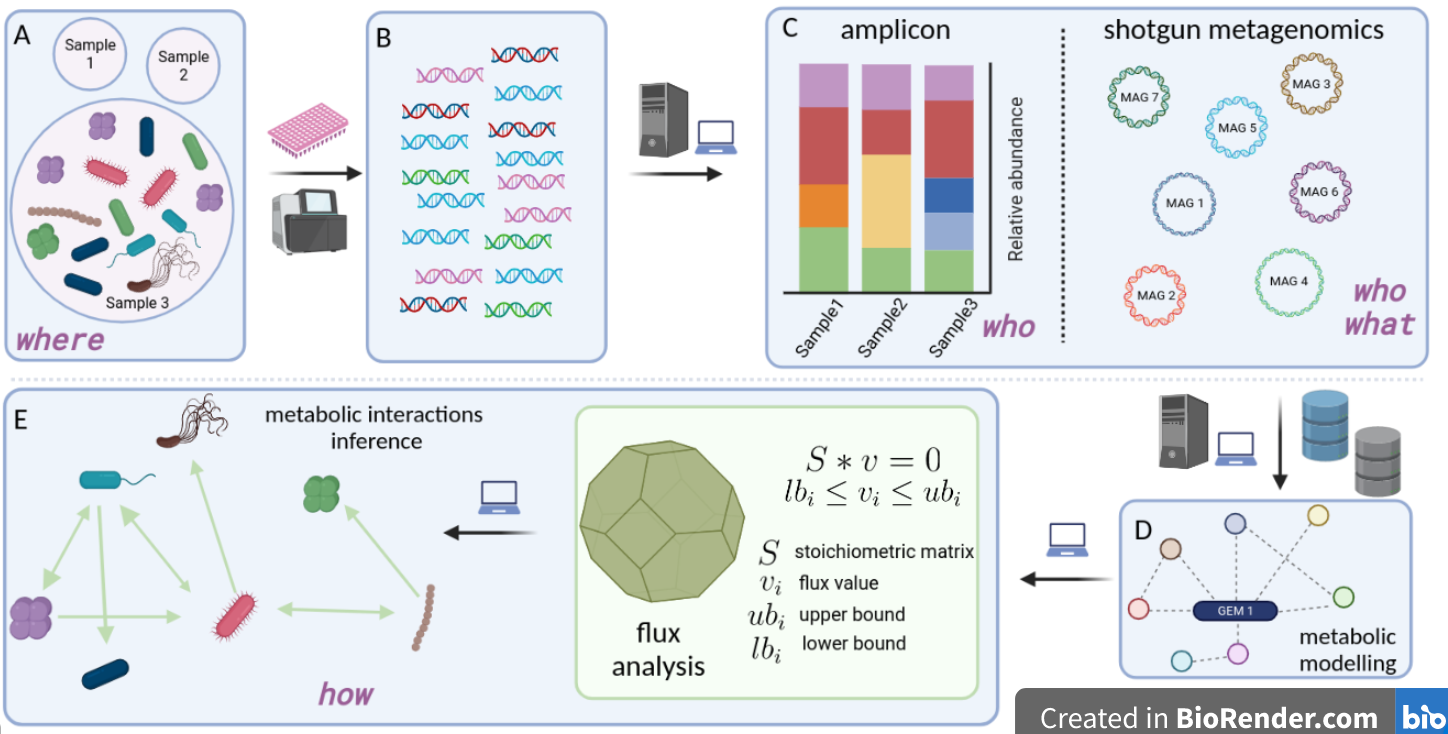
\includegraphics[width=135mm]{figures/Selection_935.png}
            \caption[Reverse ecology approach]{}
         \end{figure}
   
   


      




    


      



      % \begin{figure}[h]
      %    \centering
      %    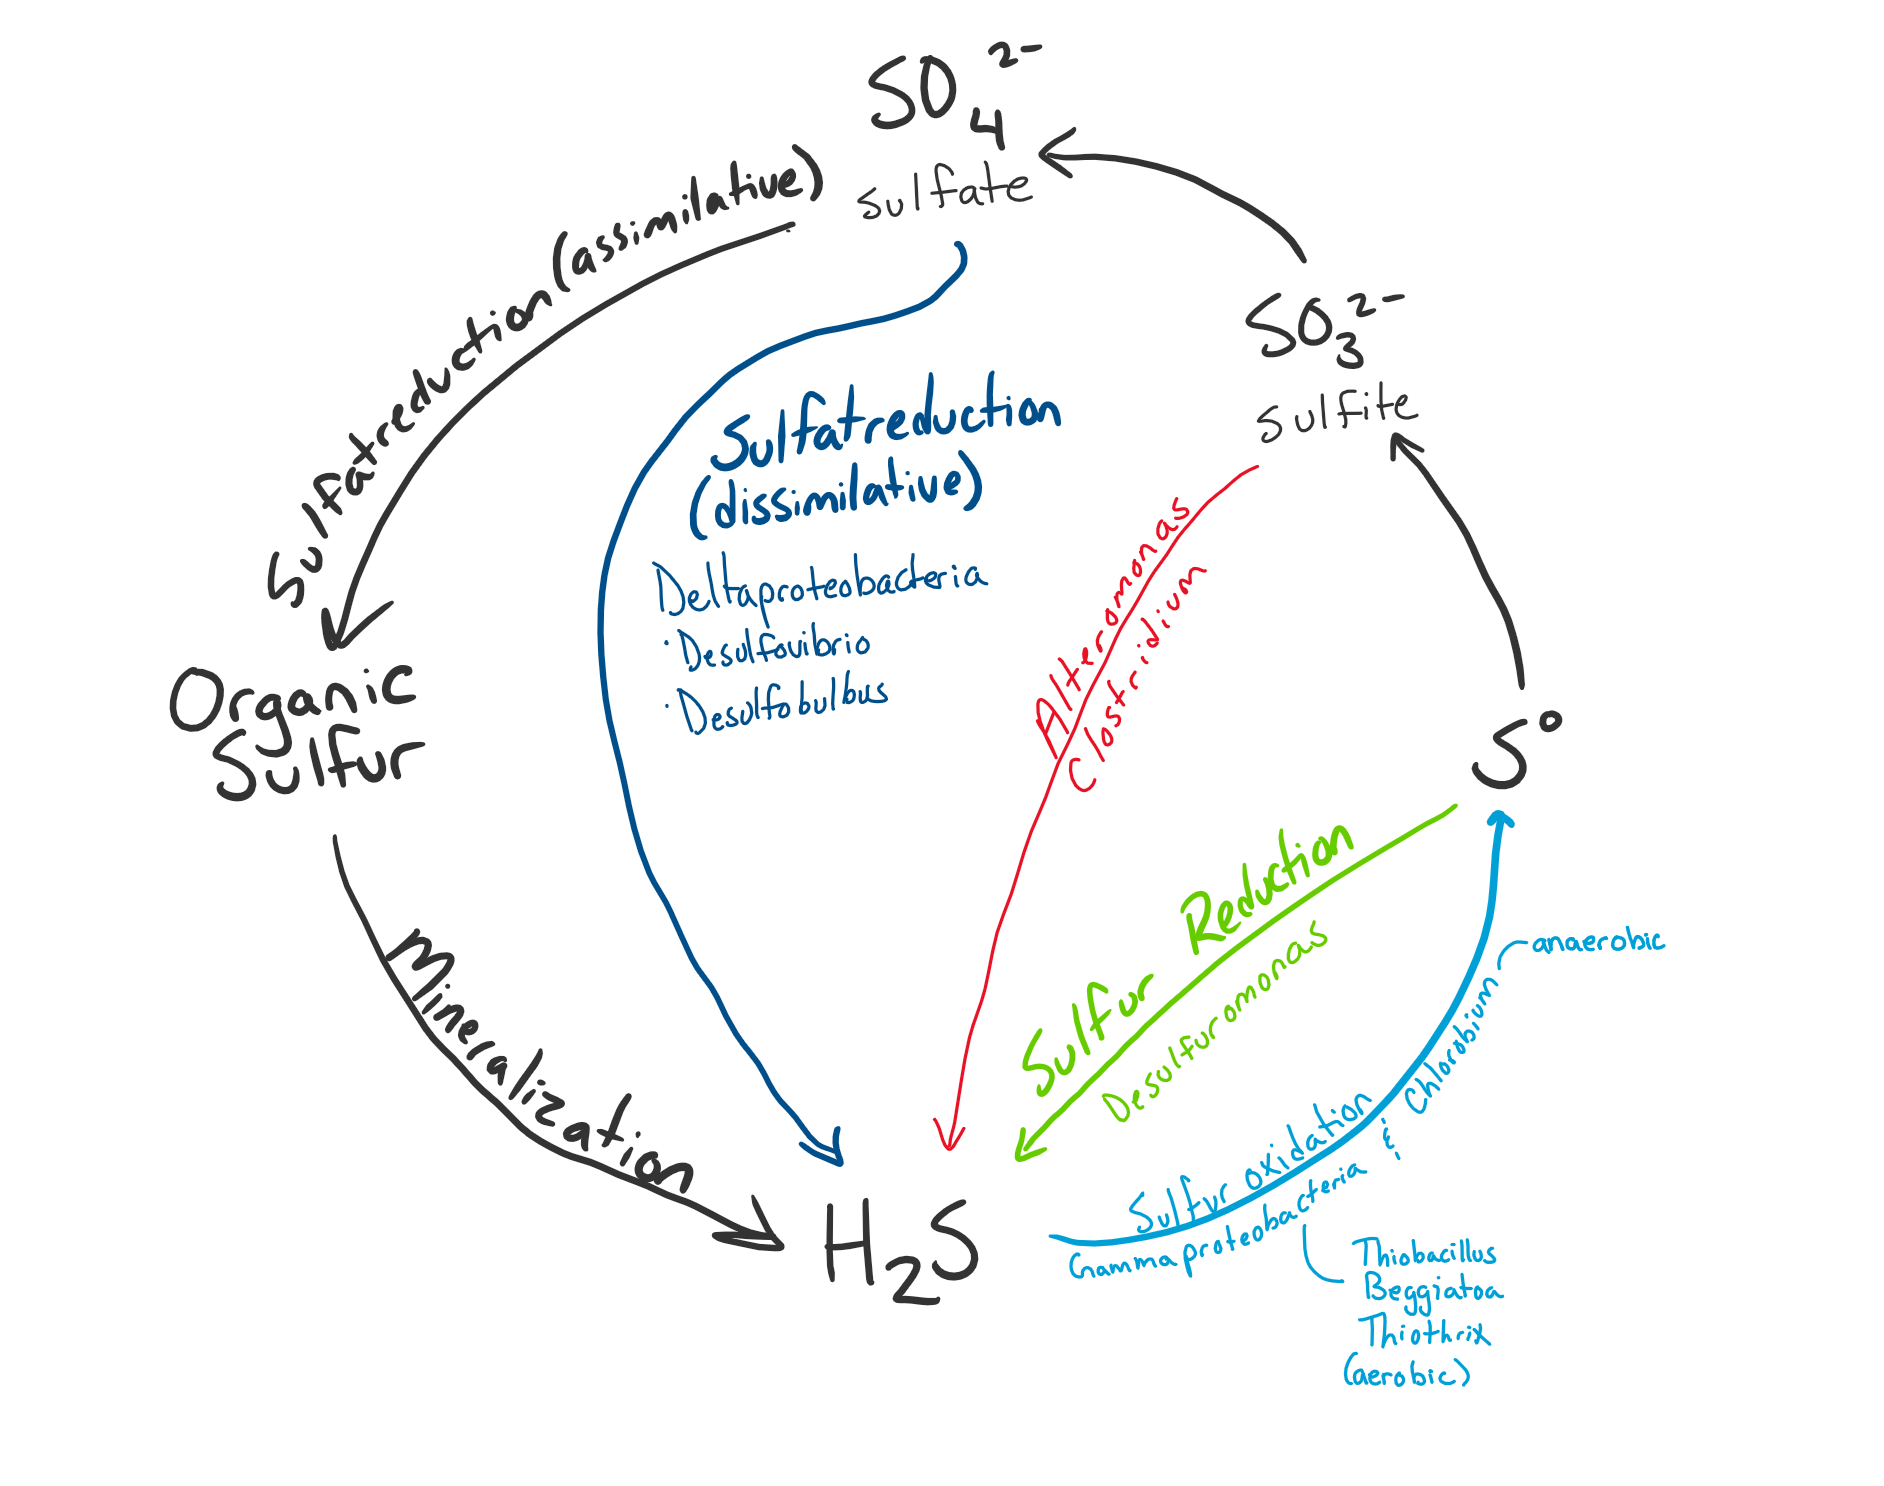
\includegraphics[width=105mm]{figures/Sulfur_Cycle_for_Hydrothermal_Vents.png}
      %    \caption[Sulfur cycle]{Sulfur cycle. Figure taken from \citep{wiki:sulfur}}
      % \end{figure}







% % SECTION 2
\section{The omics' era}

\subsection{High Throughput Sequencing approaches}

   To discover the microbial taxa present in a sample, scientists have 
   adopted multiple ways throught the years. 
   It is but a particularly limited proportion of the microbial species 
   can be cultured~\citeyear{steen2019high}.
   Therefore, monocultures and enrichment cultures allow us to observe 
   only a small fraction of the actual diversity. 
   As a consequence, other methods for the taxonomic identification of theses
   species was needed.
   development of different methods based
   on molecular analysis of microbial communities 
   To address this challenge, scientists 


   \if 0
   DNA metabarcoding is a rapidly evolving method that is being more frequently employed 
   in a range of fields, such as biodiversity, biomonitoring, molecular ecology and others 
   \citep{deiner2017environmental, ruppert2019past}. 
   Environmental DNA (eDNA) metabarcoding, targeting DNA directly isolated from environmental samples 
   (e.g., water, soil or sediment, \citep{taberlet2012environmental}), is considered a holistic 
   approach~\citep{stat2017ecosystem} in terms of biodiversity assessment, providing high detection capacity. 
   At the same time, it allows wide scale rapid bio-assessment~\citep{stat2017ecosystem} 
   at a relatively low cost as compared to traditional biodiversity survey methods~\citep{ji2013reliable}. 
   The underlying idea of the method is to take advantage of genetic markers, i.e. marker loci, using primers anchored in conserved regions. 
   These universal markers should have enough sequence variability to allow distinction among related taxa and be flanked by conserved regions allowing for universal or semi-universal primer design \citep{deagle2014dna}. 
   \fi




\subsection{Bioinformatics challenges}


   \begin{itemize}
      \item need for tools 
      \item handle the sequences 
   \end{itemize}




% SECTION 3
\section{Data integration \& data mining in the era of omics}


\subsection{Metadata: a key issue for the microbiome community}

   The Community initially focused on developing open science "best practices" for the research community. 
   The paper "The metagenomic data life-cycle: standards and best practices" \citep{ten2017metagenomic} provided the foundation for FAIR data management in the domain. 
   These best practices advocated using community standards for contextual provenance and metadata at all stages of the research data life cycle.

   Alongside archived sequence data, access to comprehensive metadata is important to contextualise where the data originated. 
   On submission, submitters are given the option to provide details regarding when, where and how their samples were collected with the opportunity to align provided metadata against community developed standards where possible. 
   However, challenges associated with metadata deposition mean submitters do not always provide comprehensive metadata - these challenges can range from: 
   lack of training and outreach resulting in submitters not fully understanding the importance of metadata and how to comply with standards; 
   as well as the trade-offs for the archives to provide complex and thorough validation vs simple user interfaces to ensure both compliance and submission are as easy as possible. 
   For the ENA, extensive documentation exists on how to submit data which both encourages compliance with metadata standards and provides separate submission guidelines for different data types - usage of the documentation can mitigate common errors and often aid first-time submitters but does not reach the full user-base. 

   FAIR principles, to provide a multilayer set of metadata required by the different scientific communities, reflecting the inherently multi-disciplinary character of environmental microbiology. 
   The various layers of metadata necessary for the FAIRification of MAGs should include:
   \begin{enumerate}
      \item Environmental data describing the sample of origin
      \item Sequencing technology or technologies
      \item Details on the computational pipeline for metagenome assembly, binning and quality assessment
      \item Connection to an existing taxonomy schema
   \end{enumerate}


   OSD’s open access strategy and provenance for metadata annotation is reflected in its ENA and Pangea submissions. 
   Among others Standardization and training are key aspects across OSD: from sampling protocols to metadata checklists and guidelines. 
   This is inline with aims of the Elixir microbiome community (see Sections "Mobilising raw data and metadata", 
   "Training - lack of training"); 
   spreading the experience to other biomes can benefit such ends.


   Open questions: 
   Metadata standard definition: minimum set and formats (Some flexibility will have to be considered in sharing standards between domain-specific communities).
   Systems to extract the vast amount of metadata locked in the scientific literature and provide them in standard format (explored by the Biodiversity Focus Group).


   Metadata associated with the raw data, the assembled data, and the workflow. The necessary scripts will be written in Python using standard libraries and Biopython. 
   Metadata of the cleaned data
   Metadata associated with the data sequencing, sample collection (MIMS), and quality control analyses will be generated according to the ENA manifest to enable uploading and archiving of the data to ENA.
   Metadata of the assembled data
   Because the workflow is distributed, it is necessary for EBI-MGnify to verify the provenance of the data workflow through registration and a verification test. A unique calculated hash generated from the data and workflow code will serve as a key for verification. This metadata will be generated at this step and together with the metadata associated with the assembly, uploaded to ENA/MGnify for further downstream functional annotation.
   Metadata to accompany the taxonomic inventories
   Metadata associated with the previous two steps will be summarised for inclusion with the taxonomic inventories (biom file format and CSV) for publication on the EMBRC GOs website.


   \begin{itemize}
      \item Metadata of the cleaned data; metadata associated with the data sequencing, sample collection (MIMS), and quality control analyses
      \item Metadata of the assembled data
      \item Metadata to accompany the taxonomic inventories

   \end{itemize}  




\subsection{Ontologies \& databases: the corner stone of mordern biology}


   Databases

   \begin{itemize}
      \item GenBank, ENA
      \item repositories such as MGnify 
      \item PubMed
   \end{itemize}


   Ontologies: 

   \begin{itemize}
      \item ENVO
      \item NCBI Taxonomy 
      \item Gene Ontology 
      \item Uniprot
      \item KEGG
      \item https://edamontology.org/page
   \end{itemize}



% SECTION 4
\section{Metabolic modeling at the omics era}

   \subsection{Genome-scale metabolic model analysis}

      The relationship between genotype and phenotype is fundamental to biology.
      Many levels of control are introduced when moving from one to the other. 
      Systems biology aims at deciphering "the strategy" both at the cell and at higher levels of organization, in case of multicell species, that enables organisms to produce orderly adaptive behavior in the face of widely varying genetic and environmental conditions (\cite{strohman2002maneuvering}); 
      the term "strategy" is used as per \cite{polanyi1968life}.
      Systems biology approaches aim at interpreting how a system's properties emerge; 
      from the cell to the community level.
      As \citeauthor{polanyi1968life} (\citeyear{polanyi1968life}) underlines 
      "live mechanisms and information in DNA are boundary conditions with a sequence of boundaries above them". 

      Being at the helm of the most critical celular functions, 
      metabolism and therefore, metabolic networks and their analysis, 
      play a key role in Systems Biology. 
      Moreover, \citeauthor{lewis2012constraining} (\citeyear{lewis2012constraining}) 
      describe thoroughly the multiple constraint-based reconstruction and analysis (COBRA) methods 
      that have been developed to support the analysis of such networks. 
   \subsection{Sampling the flux space of a metabolic model: challenges \& potential}



% SECTION 5
\section{The hypersaline Tristomo swamp: a case study of an extreme environment}


% SECTION 6
\section{Systems biology from a computational resources point-of-view}





% SECTION 7 - first draft ready
\section{Aims and objectives}

   The aim of this PhD was double:
   \begin{enumerate}
      \item to enhance the analysis of microbiome data by building algorithms and software 
            to address some of the on-going computational challenges on the field.
      \item to exploit these methods to identify taxa, functions, especially related to sulfur cycle, 
            and microbial interactions that support life in microbial community assemblages in hypersaline sediments.
   \end{enumerate}
   All parts of this work are purely computational. 
   Samples and their corresponding sequencing data used in Chapter~\ref{cha:swamp} have been collected 
   and produced by \href{https://scholar.google.com/citations?user=3zs1rNkAAAAJ&hl=en&oi=sra}{Dr. Christina Pavloudi}. 

   In \textbf{Chapter~\ref{cha:2}}, challenges derived from the analysis of HTS amplicon data are examined.
   A bioinformatics pipeline, called \texttt{pema}, for the analysis of several marker genes was developed, combinining several new technologies that allow large scale analysis of hundreds of samples. 
   In addition, a software tool called \texttt{darn}, was built to investigate the unassigned sequences in amplicon data of the COI marker gene. 

   In \textbf{Chapter~\ref{cha:prego}}, data integration, data mining and text-mining methods were exploited to build a knowledge-base, called \texttt{prego}, including millions of associations between:
   \begin{enumerate}
      \item microbial taxa and the environments they have been found in 
      \item microbial taxa and biological processes they occur
      \item environmental types and the biological processes that take place there
   \end{enumerate}

   In \textbf{Chapter~\ref{cha:dingo}}, the challenges of flux sampling in metabolic models of high dimensions was presented along with a Multiphase Monte Carlo Sampling (MMCS) algorithm we developed. 

   In \textbf{Chapter~\ref{cha:swamp}}, sediment samples from a hypersaline swamp in Tristomo, Karpathos Greece were analysed using both amplicon and shotgun metagenomics. 
   The taxonomic and the functional profiles of the microbial communities present there were investigated. 
   Key microbial interactions for the assemblages were infered. 
   All the methods developed and presented in the previous chapters were used to enhance the analysis of this microbiome.

   In \textbf{Chapter~\ref{cha:hpc}}, the history of the IMBBC-HCMR HPC facility was presented indicating the vast needs of computing resources in modern analyses in general and in microbial studies more specifically. 


   Finally, in \textbf{Chapter~\ref{cha:conclusion}}, general discussion and conclusions that have derived from this research were presented. 






%    NOTES
%    biotic interactions                  --> cross-feeding of byproduscts, competition for nutrients 
%    confounder (or 'confounding factor') --> something, other than the thing being studied, that could be causing the results seen in a study. 
%                                             confounders have the potential to change the results of research because they can influence the outcomes
%                                             that the researchers are measuring.
%                                             EXAMPLE: we found that people eating red meat have higher possibility for heart issues; but we have to 
%                                                      check whether everyone in the study who ate a lot of red meat may also have smoked cigarettes
%                                                      regularly or been overweight. 
%    circumvented                         --> shortchut, find a way around (an obstacle).
%    stratify                             --> stromatopoio // 
%    stringent                            --> austiros, strict
%    a habitat filtering model supposes that
% habitats with differing environmental
% features support non-overlapping sets of taxa
